\documentclass[9pt]{beamer}
%\include{config/commands}
%
% Choose how your presentation looks.
%
% For more themes, color themes and font themes, see:
% http://deic.uab.es/~iblanes/beamer_gallery/index_by_theme.html
%
%!TEX root = ../notas_de_clase.tex

%preamble

%language
\usepackage[spanish,es-nodecimaldot]{babel}
\usepackage[utf8]{inputenc}
\usepackage{apacite}
\usepackage[absolute,overlay]{textpos}

%packages
\usepackage[Algoritmo]{algorithm}
\usepackage{algorithmicx}
\usepackage[noend]{algpseudocode}
\usepackage{mathtools}
\setlength {\marginparwidth}{2cm}
\usepackage{todonotes}
\usepackage{amsbsy}
\usepackage{amssymb}
\usepackage{amsmath,bm}
\usepackage{dsfont}

\usepackage{xcolor}
\providecommand{\sred}[1]{\textcolor{red}{#1}}
\providecommand{\sblue}[1]{\textcolor{blue}{#1}}
\providecommand{\red}[1]{\textcolor{red}{\text{#1}}}
\providecommand{\blue}[1]{\textcolor{blue}{\text{#1}}}
\providecommand{\redb}[1]{\textcolor{red}{\textbf{#1}}}
\providecommand{\blueb}[1]{\textcolor{blue}{\textbf{#1}}}
\usepackage{graphicx}
\usepackage{fancybox}
\usepackage{booktabs}
\usepackage{caption}
\usepackage{float}
%\usepackage[longend,ruled,algochapter,linesnumbered,lined,boxed,commentsnumbered,spanish]{algorithm2e}
%\usepackage[algo2e]{algorithm2e}
\usepackage{amssymb}
\usepackage{amstext}
\usepackage{bm}
\usepackage{wrapfig}
\usepackage{subcaption} % para_unsupervised_chapter

%formatting

\usepackage[export]{adjustbox}

%caption para figuras
\captionsetup[figure]{width=.8\linewidth, font=small,labelfont={bf},name={Fig.},labelsep=period}
\captionsetup[table]{width=.8\linewidth,font=small,labelfont={bf},name={Tabla},labelsep=period}



\ifx\byn\undefined
    \definecolor{my_blue}{HTML}{C2D5FF}
    \definecolor{my_red}{HTML}{FFC2C2}
    \definecolor{my_yellow}{HTML}{FFFFE0}
\else
    \definecolor{my_blue}{HTML}{FFFFFF}
    \definecolor{my_red}{HTML}{FFFFFF}
    \definecolor{my_yellow}{HTML}{FFFFFF}
\fi


\usepackage[framemethod=TikZ]{mdframed}
\mdfdefinestyle{discusion}{%
    %linecolor=black,
    %outerlinewidth=0pt,
    roundcorner=0pt,
    innertopmargin=5pt,
    innerbottommargin=5pt,
    innerrightmargin=20pt,
    innerleftmargin=20pt,
    backgroundcolor=my_blue}

\colorlet{Green}{green!90}


\mdfdefinestyle{ejemplo}{%
    %linecolor=black,
    %outerlinewidth=0pt,
    roundcorner=0pt,
    innertopmargin=5pt,
    innerbottommargin=5pt,
    innerrightmargin=20pt,
    innerleftmargin=20pt,
    backgroundcolor=my_yellow}


\mdfdefinestyle{pendiente}{%
    style = discusion, 
    backgroundcolor=my_red}


\RequirePackage{url}



%definitions
\def\td{{\text d}}
\def\cN{{\mathcal N}}
\def\cX{{\mathcal X}} 
\def\cC{{\mathcal C}} 
\def\N{{\mathbb N}}
\def\d{{\text d}}
\def\datos{{\mathcal D}}
\def\eye{{\mathbb I}}
\def\ssum{{\scriptstyle\sum}}
\def\bepsilon{{\bm \epsilon}}
\def\tx{\tilde{x}}
\def\tX{\tilde{X}}
\def\thetaMAP{\theta_\text{MAP}}
\newcommand{\gp}{\ensuremath{\mathcal{GP}}}
\newcommand{\pr}{\ensuremath{\mathbb{P}}}
\newcommand{\x}{\ensuremath{\mathbf{x}}}
\newcommand{\z}{\ensuremath{\mathbf{z}}}
\newcommand{\cvector}{\ensuremath{\mathbf{c}}}
\newcommand{\e}{\ensuremath{\mathbf{e}}}
\newcommand{\y}{\ensuremath{\mathbf{y}}}
\newcommand{\bx}{\ensuremath{\textcolor{blue}{X}}}
\newcommand{\by}{\ensuremath{\textcolor{blue}{Y}}}
\newcommand{\rx}{\ensuremath{\textcolor{red}{X_*}}}

\newcommand{\R}{\mathbb{R}}
\newcommand{\norm}[1]{\left\lVert#1\right\rVert}




\DeclareMathOperator*{\argmax}{arg\,max}
\DeclareMathOperator*{\argmin}{arg\,min}
\DeclareMathOperator{\E}{\mathbb{E}}
\DeclareMathOperator{\V}{\mathbb{V}}
\DeclareMathOperator{\KL}{\text{KL}}
\DeclareMathOperator{\MVN}{\text{MVN}}
\newcommand\deq{\stackrel{\mathclap{\normalfont\mbox{\tiny def}}}{=}}
%\newcommand{\E}[1]{\mathbb E \left[#1\right]}
\newcommand{\trace}[1]{\text{Tr} \left[#1\right]}


\usepackage{amsthm}

%-------------------------------------------
% Newtheorem
%-------------------------------------------
\newtheorem{axioma}{\textcolor{red}{Axioma}}
\newtheorem{definicion}{Definición}
\newtheorem*{notacion}{Notación}
\newtheorem{teorema}{Teorema}
\newtheorem{corolario}{Corolario}
\newtheorem{lema}{Lema}
\newtheorem{lemaZ}{\textcolor{red}{Lema}}
\newtheorem{propiedad}{Propiedad:}
\newtheorem{proposicion}{Proposición:}
\newtheorem*{observacion}{Observación}
\newtheorem*{comentario}{Comentario}
\newtheorem*{ejemplo}{Ejemplo}
\newtheorem*{resultado}{Resultado}
\newtheorem*{propuesto}{Ejercicio propuesto}
\newtheorem*{demostracion}{Demostración} % No se usa, usar \begin{proof}\end{proof} que son por default.

%listing paackage para código
\usepackage{listings}
\usepackage{xcolor}
 
\definecolor{codegreen}{rgb}{0,0.6,0}
\definecolor{codegray}{rgb}{0.5,0.5,0.5}
\definecolor{codepurple}{rgb}{0.58,0,0.82}
\definecolor{backcolour}{rgb}{0.95,0.95,0.92}
 
\lstdefinestyle{mystyle}{
    xleftmargin=0.15\textwidth,
    linewidth=0.8\textwidth,
    backgroundcolor=\color{backcolour},   
    commentstyle=\color{codegreen},
    keywordstyle=\color{magenta},
    numberstyle=\tiny\color{codegray},
    stringstyle=\color{codepurple},
    basicstyle=\ttfamily\footnotesize,
    breakatwhitespace=true,         
    breaklines=true,                 
    captionpos=b,                    
    keepspaces=true,                 
    numbers=left,                    
    numbersep=5pt,                  
    showspaces=false,                
    showstringspaces=false,
    showtabs=false,                  
    tabsize=2
}
 
\lstset{style=mystyle}

\numberwithin{equation}{section}

\usetheme{simple}

% \usepackage[T1]{fontenc} %Este es el mismo utilizado en el tex de clases salvo modificaciones
\title{Clase 9 - Clasificación no Lineal}
\subtitle{Aprendizaje de Máquinas - MA5204}
\date{\today}
\author{Felipe Tobar} 
\titlegraphic{
\begin{figure}[htp] 
    \centering
        
\includegraphics[width=0.15\textwidth]{../img/Uchile.pdf}%
    %\hspace{2em}% 
    %    \includegraphics[width=0.15\textwidth]{img/CMM.pdf}%
         
\end{figure}
}
\institute{Department of Mathematical Engineering \&\\ Center for Mathematical Modelling\\Universidad de Chile}
%-------------------------------------------
% Inicio del documento, no tocar la config. de portada
%-------------------------------------------
\begin{document}
% Portada
\begin{frame}
  \titlepage
\end{frame}
% Tabla de contenidos
\begin{frame}{Contenido}
  \tableofcontents
  
\end{frame}
% Portada de seccion
\AtBeginSection[]{
  \begin{frame}
  \vfill
  \centering
  \begin{beamercolorbox}[sep=8pt,center,shadow=true,rounded=true]{title}
    \usebeamerfont{title}\insertsectionhead\par
  \end{beamercolorbox}
  \vfill
  \end{frame}}

%tcolorbox
%-------------------------------------------
% Contenido
%-------------------------------------------
% Nueva sección, o capitulo, tiene diapo de portada propio, basta con ponerla fuera del entorno frame
\section{El perceptrón}

\begin{frame}{El perceptrón - Introducción}
Las nociones básicas que hemos visto hasta ahora para lidiar con el problema de clasificación tienen dos problemas conceptuales. \pause
\begin{enumerate}
  \item Falta de una métrica correcta \pause
  \item No existe una \emph{función de verosimilitud} apropiada \pause
\end{enumerate}
La incorporación de esta función que conecta el modelo lineal con la clase, resulta en un \emph{modelo lineal generalizado}, es decir, una modelo lineal conectado a una  función no-lineal que llamaremos \emph{función de enlace}.\\ \pause
Sin embargo, el desafío más importante en esta construcción es que el modelo resultante ya no es lineal, ni en la entrada ni en los parámetros , pues una verosimilitud (función de enlace) lineal nunca nos llevará de un espacio de inputs (hemos asumido $\R^M$) al espacio de categorías $\{\cC_1,\cC_2,\ldots,\cC_k\}$, es decir, necesitamos una no-linealidad ``después'' de la parte lineal \\ \pause

Una forma de resolver estas problemáticas es mediante el uso del \emph{Perceptrón} \cite{rosenblatt_1958}, un modelo de clasificación binario que tuvo mucha importancia en el área de reconocimiento de patrones.

\end{frame}

\begin{frame}{El perceptrón}

El Perceptrón consiste en una función no lineal fija usada para transformar $x$ en un vector de características\footnote{En este caso consideramos no linealidad antes y después de la parte lineal, sin embargo, considerar la entrada como $x$ o  como $\phi(x)$ es  equivalente en base a lo  visto en los modelos lineales en los parámetros. } $\phi(x)\in\R^D$, que luego es usado para generar un modelo lineal \emph{generalizado} con función de enlace no lineal $f(\cdot)$ de la siguiente forma:
\begin{align*}
  y(x) &= f(\theta^\top\phi(x))\\
  f(u) &= \left\{\begin{matrix}
  +1,\quad u\geq 0\\
  -1,\quad u<0
  \end{matrix}\right.
\end{align*} \pause
El Perceptrón entonces asigna $x$ a la clase $\mathcal{C}_1$ si $y(x)=+1$ y asignará $x$ a la clase $\mathcal{C}_2$ cuando $y(x)=-1$. Notemos que  para  el caso que $\phi$ es lineal, este es el mismo clasificador presentado en la Sección de clasificación lineal, pero en este caso el criterio para asignar la clase es \textbf{parte del modelo}. \pause

Usando el hecho que las etiquetas están representadas por la  codificación $t\in\{1,-1\}$, la condición de asignación puede ser cubiertas por la expresión:
\begin{equation*}
  \theta^\top\phi(x_n)t_n > 0,\quad \forall (x_n,t_n) \in \datos.
\end{equation*}

\end{frame}

\begin{frame}{El perceptrón}
Podemos entonces satisfacer esta restricción mediante el ``criterio del perceptrón'', el cual se basa en examinar  los elementos de $\datos$ que fueron clasificados incorrectamente. Este criterio asocia a los puntos clasificados correctamente error 0 y a los puntos mal clasificados error $-\theta^\top\phi(x)t>0$. De esta forma, si denotamos $\mathcal{M}$ el conjunto de puntos mal clasificados, se debe minimizar la siguiente función objetivo: \pause 

\begin{equation*}
  J_\text{P}(\theta,x) = \E\left(-\theta^\top\phi(x)t(x)\mathds{1}_{\theta^\top\phi(x)t(x)\leq 0} \right) 
\end{equation*} \pause
\begin{equation*}
\approx -\sum_{(x_i,t_i)\in \mathcal{D}}\theta^\top\phi(x_i)t_i \mathds{1}_{\theta^\top\phi(x_i)t_i\leq 0} = -\sum_{(x_i,t_i)\in \mathcal{M}}\theta^\top\phi(x_i)t_i
\end{equation*} 

Para el problema de minimización del funcional del perceptrón, se puede utilizar el método del gradiente estocástico.

\end{frame}

\begin{frame}{Método del gradiente estocástico}


En aprendizaje de máquinas por lo general se busca un parámetro óptimo que minimice el error de ajuste de acuerdo a una función de pérdida $J$. Dicho problema puede ser escrito de la forma: \pause
  
  \begin{equation*}
    \hat{\theta} = \argmin_\theta \sum_{i=1}^n J(y_i,\hat{y}_\theta(x_i)) = \argmin_\theta \frac{1}{n} \sum_{i=1}^n J(y_i,\hat{y}_\theta(x_i))
  \end{equation*} \pause 
  
  Donde $y_i$ corresponde a la salida de $x_i$ mientras que $\hat{y}_\theta(x_i)$ representa la predicción de la salida de $x_i$ mediante un modelo de parámetro(s) $\theta$.\\ \pause 
  
  Muchas veces es infactible encontrar el óptimo de forma analítica o bien, el algoritmo del gradiente clásico se queda atrapado en mínimos locales. Una forma distinta de ver el problema es considerar que $(x_i,y_i)\sim\mu$ iid para una distribución $\mu$ desconocida. Desde ese punto de vista, el problema se reduce a minimizar $\E\left(J(y,\hat{y}_\theta(x))\right)$. Este tipo de problemas puede ser escrito en general como \pause 
  
  \begin{equation*}
    \min_\theta \E(f(\theta,X)),\quad X\sim \mu\text{ desconocida}
  \end{equation*} 




\end{frame}


\begin{frame}{Método del gradiente estocástico }
Una alternativa al método del gradiente clásico $\theta^{\tau+1} = \theta^\tau - \beta_{\tau+1}\nabla_\theta \E(f(\theta^\tau,X))$ consiste en utilizar las observaciones iid $(x_i)_{i\geq 1}\sim\mu$ al momento de iterar, considerando una observación por iteración en vez del funcional $\E(f(\theta^\tau,X))$ completo, es decir: \pause 

\begin{equation*}
  \theta^{\tau+1} = \theta^\tau - \eta_{\tau+1}\nabla_\theta f(\theta^\tau,x_{\tau+1})
\end{equation*} \pause 

Notar que en cada iteración se necesita evaluar una sola vez $\nabla_\theta f$ y no hace falta calcular su esperanza, más aún, este algoritmo permite entrenar modelos con datos a medida que van llegando (actualización a tiempo real) \\ \pause 

Este algoritmo es conocido como método del gradiente estocástico (SGD), donde el término $\nabla_\theta f(\theta^\tau,x_{\tau+1})$ puede ser visto como un gradiente exacto perturbado: \pause 

\begin{equation*}
  \nabla_\theta f(\theta^\tau,x_{\tau+1}) = \nabla_\theta\E(f(\theta^\tau,X)) + \Delta_t
\end{equation*} \pause 

Donde $\Delta_t = \nabla_\theta f(\theta^\tau,x_{\tau+1}) - \nabla_\theta \E( f(\theta^\tau,X))$ cumple que $\E(\Delta_t)=0$ ya que de acuerdo a la regla integral de Leibniz, $\nabla_\theta \E( f(\theta^\tau,X)) =  \E(\nabla_\theta f(\theta^\tau,X))$.\\ \pause


Esta propiedad del gradiente con ruido es la que le permite al algoritmo del gradiente estocástico poder saltarse con mayor facilidad los mínimos locales ya que la evolución de $\theta_\tau$ contiene una parte aleatoria que no depende del valor del gradiente en el punto.


\end{frame}

\begin{frame}{Método del gradiente estocástico}

\begin{figure}[H]
  \centering
  \visible<1->{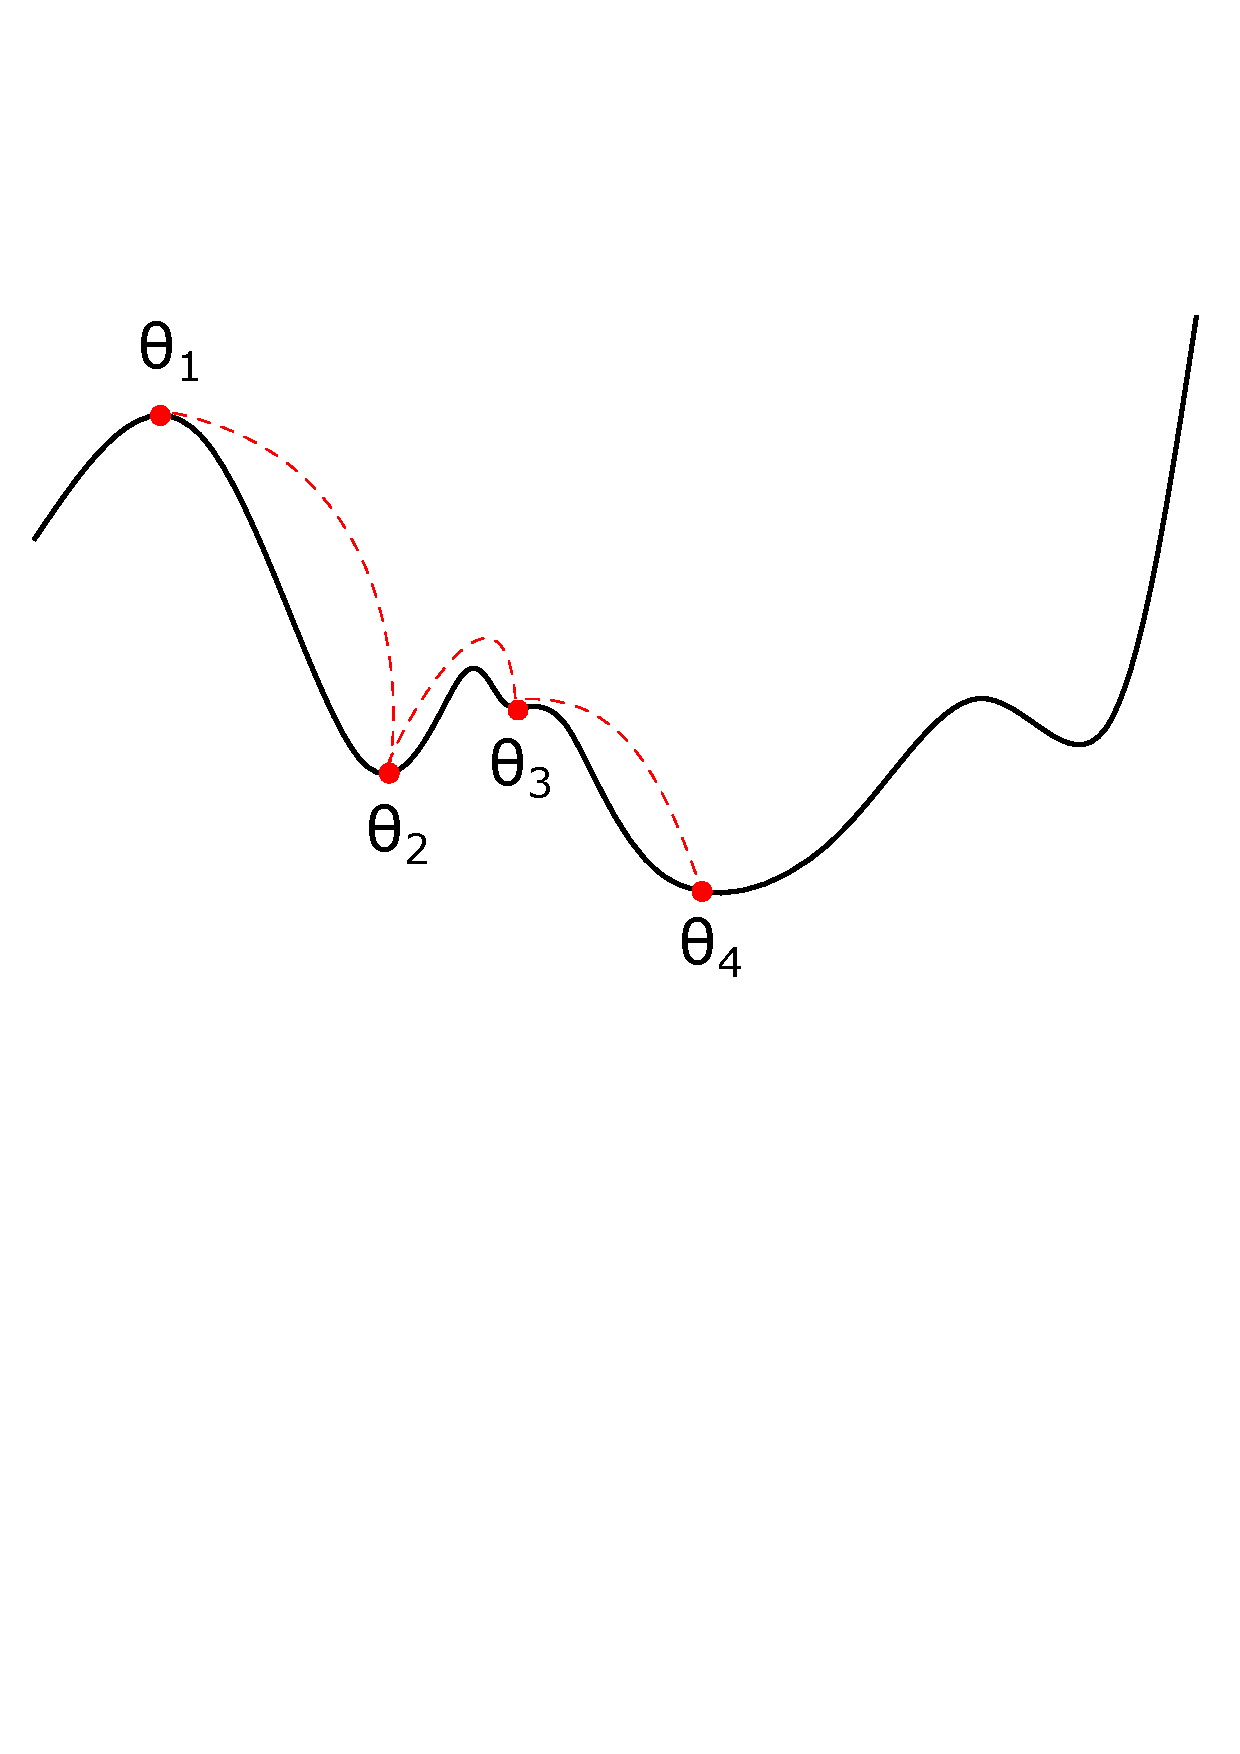
\includegraphics[width=0.5\textwidth]{../img/cap3_sgd.pdf}}\\
  \caption{Posibles iteraciones del algoritmo SGD. El algoritmo del gradiente clásico hubiese quedado atrapado en $\theta_2$ ya que en dicho punto el gradiente es nulo por lo que no hay desplazamiento.}
\end{figure} \pause 

\begin{theorem}[Sigmund-Robins] Bajo hipótesis razonables sobre $f$ (regularidad en $\theta$, integrabilidad de $\nabla_\theta f$ y cotas) y tasas de aprendizaje suficientemente pequeñas (por ejemplo, $\eta_\tau = 1/\tau$), la sucesión $(\theta^\tau)_{\tau\geq 1}$ converge c.s. al conjunto de puntos críticos de $\E(f(\theta,X))$.\\   
  \end{theorem}



\end{frame}








\begin{frame}{El perceptrón}

En este caso, el algoritmo iterativo tiene la siguiente estructura: \pause
\begin{align*}
  \theta^{\tau+1} &= \theta^\tau - \eta_\tau \nabla_\theta J_\text{P}(\theta^\tau,x_i)\nonumber\\
  &= \theta^\tau + \eta_\tau \phi(x_i)t_i.\label{eq:percetron_rule}
\end{align*}\pause
Es importante notar que al actualizar el vector $\theta$, el conjunto de puntos mal clasificados $\mathcal{M}$ va a cambiar, pues (esperamos que) en cada iteración los elementos del conjunto de puntos mal clasificados vaya disminuyendo.\\

Por lo tanto, el algoritmo de entrenamiento para el perceptrón es el siguiente: \pause

\begin{itemize}
  \item[i)] se recorre el conjunto de puntos de entrenamiento $\{x_i\}_{i=1}^N$, \pause
  \item[ii)] si el punto $x_i$ fue clasificado correctamente el vector de pesos de mantiene igual \pause
  \item[iii)] si $x_i$ fue clasificado incorrectamente, el vector $\theta^\tau$ es actualizado según la ecuación anterior con $\eta=1$ mediante
  \begin{equation*}
   \theta^{\tau+1} = \theta^\tau + \phi(x_i)t_i.
  \end{equation*} 
\end{itemize}
\pause
Es decir, el parámetro $\theta$ está paso a paso modificado en la dirección de las características $\phi(x_i)$ con multiplicador $\pm1$ en base a la clase verdadera de $x_i$ hasta  que todos los puntos de $\datos$ están bien clasificados.


\end{frame}
\section{Clasificación probabilística: modelo generativo}

\begin{frame}{Modelo generativo}
Los modelos que hemos revisado hasta este punto son del tipo \emph{discriminativo}, es decir, modelan directamente la función $f:x\mapsto c$. Con una interpretación probabilística, esto es equivalente a modelar la probabilidad condicional $\mathbb{P}(\mathcal{C}_k|x)$, es decir, dado que conozco el input (o características de) $x$, cuál es la distribución de probabilidad sobre las clases. Sin embargo, hemos considerado métodos determinísticos, que solo asignan probabilidad 1 a una sola clase. \pause
\vspace{0.5cm}

Un paradigma alternativo es considerar es un enfoque \emph{generativo}, en el cual modelamos dos  objetos: en primer lugar la ``probabilidad condicional de clase'' la cual representa cómo distribuyen los valores de los inputs $x$ cuando la  clase es, por  ejemplo, $\cC_k$, denotada por $\mathbb{P}(x|\mathcal{C}_k)$. En segundo lugar las ``probabilidades de clase'', o el prior sobre clases, denotada $\mathbb{P}(\mathcal{C}_k)$. Luego, podemos calcular la densidad posterior sobre las clases dado un input $x$ usando el Teorema de Bayes de acuerdo a 
\begin{equation*}
  \mathbb{P}(\mathcal{C}_k|x) = \frac{\mathbb{P}(x|\mathcal{C}_k)\mathbb{P}(\mathcal{C}_k)}{\mathbb{P}(x)}.
\end{equation*}

\end{frame}

\begin{frame}{Modelo generativo}
Para el caso de 2 clases, se tiene el siguiente desarrollo: \pause 
\begin{align*}
  \mathbb{P}(\mathcal{C}_1|x) 
  &= \frac{\mathbb{P}(x|\mathcal{C}_1)\mathbb{P}(\mathcal{C}_1)}{\mathbb{P}(x)}\nonumber\\
  &= \frac{\mathbb{P}(x|\mathcal{C}_1)\mathbb{P}(\mathcal{C}_1)}{\mathbb{P}(x|\mathcal{C}_1)\mathbb{P}(\mathcal{C}_1)+\mathbb{P}(x|\mathcal{C}_2)\mathbb{P}(\mathcal{C}_2)}\nonumber\\
  &=\frac{1}{1+\frac{\mathbb{P}(x|\mathcal{C}_2)\mathbb{P}(\mathcal{C}_2)}{\mathbb{P}(x|\mathcal{C}_1)\mathbb{P}(\mathcal{C}_1)}}\nonumber\\
  &=\frac{1}{1+\exp(-r)} = \sigma(r).\label{eq:logistic1}
\end{align*} \pause 
Donde hemos introducido la notación $r = r(x) =\ln\left(\frac{\mathbb{P}(x|\mathcal{C}_1)\mathbb{P}(\mathcal{C}_1)}{\mathbb{P}(x|\mathcal{C}_2)\mathbb{P}(\mathcal{C}_2)}\right)$  y la  función logística definida mediante $\sigma(r) = \frac{1}{1+e^{-r}}$, la cual  tiene propiedades que serán útiles en el entrenamiento, en particular: \pause
\begin{align*}
  \text{reflejo: }\sigma(-r)&=1-\sigma(r)\\
  \text{derivada: }\frac{d}{dr}\sigma(r)&=\sigma(r)(1-\sigma(r))\\
  \text{inversa: }r(\sigma)&=\ln\left(\frac{\sigma}{1-\sigma}\right).
\end{align*}


\end{frame}

\begin{frame}{Modelo generativo}
Si bien la expresión de la distribución condicional en la ecuación anterior parece una presentación antojadiza para hacer aparecer la  función logística (sigmoide), pues $r=r(x)$ puede ser cualquier cosa. Sin embargo, veremos que existe una elección particular de las distribuciones condicionales de clase que lleva a un $r$ que es efectivamente lineal en $x$. En general, nos  referiremos a este clasificador como \textbf{regresión logística} en dicho caso, es decir, cuando $r(x) = a^\top x  + b$. \pause

Podemos ahora considerar el caso de múltiples clases $\{\cC_1,\ldots,\cC_K\}$, donde un desarrollo similar al anterior resulta en:  
\begin{equation*}
  \mathbb{P}(\mathcal{C}_i | x) = \frac{\mathbb{P}(x | \mathcal{C}_i)\mathbb{P}(\mathcal{C}_i)}{\sum_{j}\mathbb{P}(x | \mathcal{C}_j)\mathbb{P}(\mathcal{C}_j)} = \frac{\exp(s_i)}{\sum_{j}\exp(s_j)},\label{eq:softmax1}  
\end{equation*}
\pause
donde hemos denotado $s_i = \log\left(\mathbb{P}(x | \mathcal{C}_i)\mathbb{P}(\mathcal{C}_i)\right)$. La función que aparece al lado derecho de la ecuación se conoce como \emph{exponencial normalizada} o \emph{softmax}, y corresponde a una generalización de la función logística a múltiples clases. \\Además, esta función tiene la propiedad de ser una aproximación suave de la función máximo y convertir cualquier vector $s=[s_1,\ldots,s_k]$ en una distribución de probabilidad, donde podemos hablar de ``la probabilidad de ser clase $\cC_k$''.


\end{frame}

\begin{frame}
  \titlepage
\end{frame}

%Quitar de comentarios apenas se agregue alguna referencia 
\bibliography{../capitulos/referencias} %Bibliografía
\bibliographystyle{apacite}
\end{document} 